\subsection{Glyph: \glyph{Not}}\label{sec:not}

\corr{The glyph \glyph{not} is used to denote that the \glyph{EPN} linked as input cannot produce the output.}
{
The output of a \glyph{not} glyph is True if its input is False, and False otherwise.
}

\begin{glyphDescription}

\glyphSboTerm
SBO:0000238 ! not

\corr{
\glyphOrigin One \glyph{EPN} (section~\ref{sec:EPNs}) or \glyph{logical operator} (section~\ref{sec:logic}).
}{
\glyphIncoming One \glyph{logic arc} (\sect{logicArc}).
}

\corr{
\glyphTarget  One modulation (section~\ref{sec:modulation}), stimulation (section~\ref{sec:stimulation}), catalysis (section~\ref{sec:catalysis}), inhibition (section~\ref{sec:inhibition}) or necessary stimulation (section~\ref{sec:necessary_stim}) arc.
}{
\glyphOutgoing
One \glyph{logic arc} (\sect{logicArc}) or \glyph{modulation arc} (\sect{modulations}).
}

\glyphContainer
A \glyph{not} operator is represented by a circular shape containing the word ``NOT''.
The shape is linked to two ports, that are small arcs attached to the centres of opposite sides of the shape, as shown in \fig{not}.
The incoming \glyph{logic arc} (\sect{logicArc}) is linked to the extremity of the leftmost or uppermost port, while the outgoing \glyph{logic arc} (\sect{logicArc}) or \glyph{modulation} (\sect{modulation}) is linked to the extremity of the rightmost or bottommost port.

\glyphLabel
\corr{A \glyph{not} operator is not identified by any label}{None}.

\glyphAux
\corr{A \glyph{not} operator does not carry any auxiliary items}{None}.

\end{glyphDescription}

\begin{figure}[H]
  \centering
  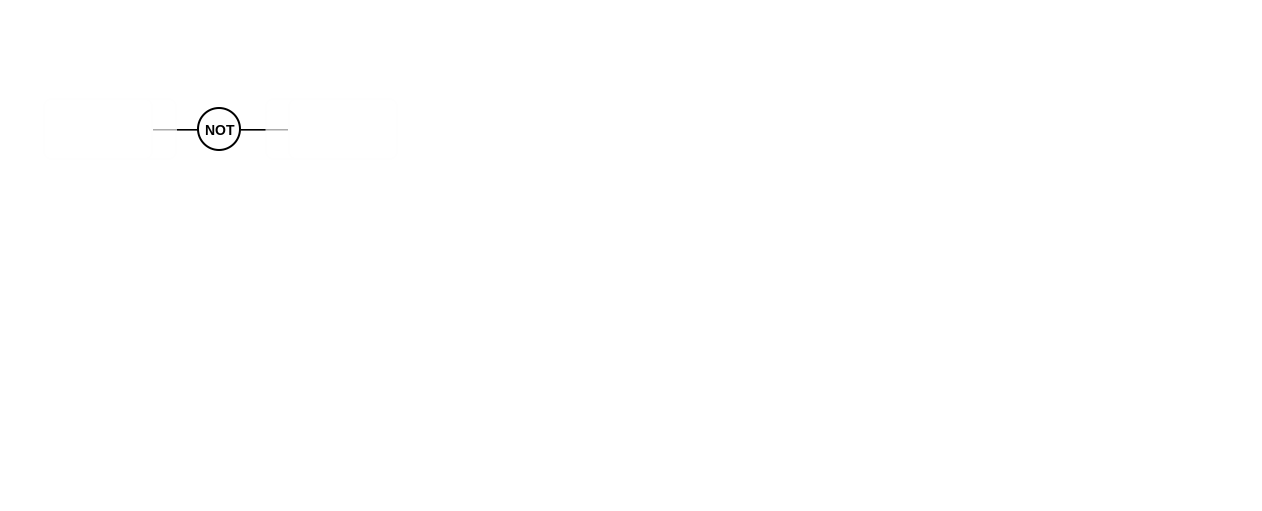
\includegraphics{images/not}
  \caption{The \PD glyph for \glyph{not}.}
  \label{fig:not}
\end{figure}
